% !TeX spellcheck = en_US
\documentclass[class=article,crop=false]{standalone}
\usepackage{pacco}
\begin{document}
\section{The Fast Fourier Transform}
\subsection{Theoretical framework}
The Fourier integral is defined\footnote{\cite{FFTbook}, p.9} as
\begin{equation}\label{ft}
F(\omega)=\int_{-\infty}^{\infty}f(x)e^{-i2\pi\omega x}\dif x.
\end{equation}
If the integral exists for every value of the parameter $\omega$, then Eq.\ref{ft} defines $F(\omega)$, the \enf{Fourier Transform} of $f(x)$. In most cases\footnote{\cite{FFTbook}, \textit{ibidem}} (including the application of our discussion), $f(x)$ is a function of the variable time and $F(\omega)$ is a function of the variable frequency. In general, the Fourier Transform is a complex quantity
\begin{equation}\label{decomp}
	F(\omega)=R(\omega)+iI(\omega)=|F(\omega)|e^{i\theta(\omega)}
\end{equation}
with;
\begin{itemize}
	\item $R(\omega)$ is the real part of the Fourier transform;
	\item $I(\omega)$ is the imaginary part;
	\item $|F(\omega)|$ is the \textit{amplitude} or \textit{Fourier spectrum} og $f(x)$ given by $\sqrt{R^2(\omega)+I^2(\omega)}$;
	\item $\theta(\omega)$ is the \textit{phase angle of the Fourier transform} and is given by $tan^{-1}\left[\frac{I(\omega)}{R(\omega)}\right]$.
\end{itemize}
In the same fashion we can define the \enf{inverse Fourier transform} as:
\begin{equation}\label{ivft}
	f(x)=\int_{-\infty}^{\infty}F(\omega)e^{i2\pi\omega x}\dif \omega.
\end{equation}
Eq.\ref{ivft} allows the determination of a function in the time domain from its Fourier transform. If the functions $f(x)$ and $F(\omega)$ are related by Eqs. \ref{ft} and \ref{ivft}, then the two function are called a \enf{Fourier transform pair} and are notated \[f(x)\xleftrightarrow{\text{FT}}F(\omega)\].\par
The Fourier transform is defined on continuous functions, but since we will be dealing with sampled (and therefore continuous) quantities, we will need to turn to the discrete version fo the Fourier transform, the \enf{Discrete Fourier transform (DFT)}\footnote{\cite{FFTbook}, chap. 6.3 provides more formal details about the connection between Fourier transform and discrete Fourer transform and its derivation.}. The DFT maps a sequence $x_n$ to a sequence $X_n$ and is defined as:
\begin{equation}\label{dft}
	X_k=\sum_{k=0}^{N-1}x_ne^{-i\frac{2\pi}{N}kn}\qquad \text{for }k=0,1,2,\ldots,N-1
\end{equation}
or, commonly\footcite[][2]{family}
\begin{equation}
	X_k=\sum_{k=0}^{N-1}x_nW_{N}^{kn}\qquad\text{with }W_n=e^{-i\frac{2\pi}{N}}.
\end{equation}
In FFT literature, this factor $W_N$ is called \textit{twiddle factor}\footcite[][565]{fftfunprofit}.\par
It is worth noting that $W_n^k$ for $k=0,\ldots,N-1$ are the \textit{Nth roots of unity}. Every twiddle factor "rotates" each input component clockwise around the complex circle. This implies that the twiddle factors are periodic with period $N$ and multiplying $W_N$ for $2\pi$ equals to no rotation at all.\\
The \enf{inverse discrete Fourier transform (IDFT)} is defined as:
\begin{equation}\label{idft}
	x_n=\frac{1}{N}\sum_{i=0}^{N-1}W_N^{kn}X_k \qquad \text{for }n=0,1,2,\ldots,N-1.
\end{equation}
If two functions are linked by Eqs. \ref{dft} and \ref{idft} they are said to be a \enf{discrete Fourier transform pair} and are notated \[x(n)\xleftrightarrow[N]{\text{DFT}}X(k)\] where $N$ represents the point in the DFT.\par
The DFT enjoys the following useful properties\footcite[][410]{dspprinciples}, extendend from the properties of the Fourier transform:
\begin{itemize}
	\item \enf{linearity}: if $x_1(n)\xleftrightarrow[N]{\text{DFT}}X_1(k)$ and $x_2(n)\xleftrightarrow[N]{\text{DFT}}X_2(k)$ then for any real-valued of complex-valued constants $a_1$ and $a_2$:
	\begin{equation}
		a_1x_1(n)+a_2x_2(n)\xleftrightarrow[N]{\text{DFT}}a_1X_1(k)+a_2X_2(k);
	\end{equation}
	\item \enf{periodicity}: if $x(n)\xleftrightarrow[N]{\text{DFT}}X(k)$ then
	\begin{align*}
		x(n+N)&=x(n)\qquad\forall n\\
		X(k+N)&=X(k)\qquad\forall k
	\end{align*}
	\item \enf{complex-conjugate properties}: consider the $k-th$ bin of the transformed sequence, with $1\leqslant k\leqslant N-1$
	$$ X_k =\sum_{n=0}^{N-1}x_ne^{-i\frac{2\pi}{N}kn}$$
	and the $(N-k)-th$ bin 
	\begin{align*}
		X_{N-k}&=\sum_{n=0}^{N-1}x_ne^{-i\frac{2\pi}{N}(N-k)n}\\
		&=\sum_{n=0}^{N-1}x_ne^{(-i2\pi+i\frac{2\pi}{N}k)n}\\
		&=\sum_{n=0}^{N-1}x_ne^{+i\frac{2\pi}{N}kn}\\
	\end{align*}
	Consider now the complex conjugate of $X_k$, $(X_k)^*$:
	\begin{align*}
		(X_k)^*&=\left(\sum_{n=0}^{N-1}x_ne^{-i\frac{2\pi}{N}kn}\right)^*\\
		&=\sum_{n=0}^{N-1}(x_n)^*e^{+i\frac{2\pi}{N}kn}
	\end{align*}
	if $x_n$ is real (and therefore has no imaginary part), we have that $(x_n)^*=x_n$ and so
	\begin{align*}
		(X_k)^*&=\sum_{n=0}^{N-1}x_ne^{+i\frac{2\pi}{N}kn}\\
		&=X_{N-k}=X(-k).
	\end{align*}
	Consequenty, 
	\[
	|X(N-k)|=|X(k)|\qquad\text{and}\qquad\angle X(N-k)=-\angle X(k)
	\]
	The fact that $X_{N-k}=(X_k)^*$ has therefore the important consequence that the real parts of $X_{N-k}$ and $X_k$ are identical, while their imaginary parts have the same maginitude but opposite signs. 
	\item \enf{time shifting}: if $x(n)$ is shifted by the integer $m$, then
	\[x(n-m)\xleftrightarrow[N]{\text{DFT}}X(k)e^{-i\frac{2\pi}{N}nm}.\] This means that any shifting in the time domain will affect the transformed element by an "adjusting" factor that rotates it appropriately around the complex circle.
	\item \enf{frequency shifting}: if $X(k)$ is shifted by the integer $m$, then
	\[x(n)e^{i\frac{2\pi}{N}km}\xleftrightarrow[N]{\text{DFT}}X(k-m).\] The same remark of time shifting can be made by switching the role of transformed and original component.
\end{itemize}
Let's now see an example for $N=4$. \par
\begin{example}
Our input will be given by the one dimensional vector $$\mathbf{\bar{x}}=[x_0,x_1,x_2,x_3].$$ Since $N=4$, we can calculate our base twiddle factor
$$W_4=e^{-i\frac{2\pi}{4}}=-i.$$ This corresponds to the 4 unitary roots in the complex plane:
\begin{figure}[H]
	\centering
	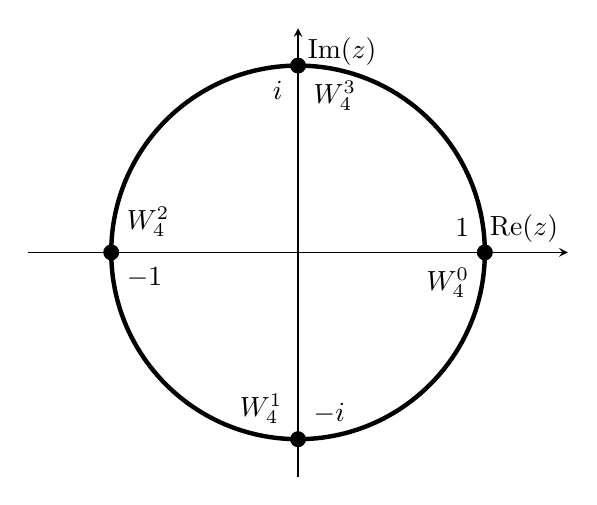
\begin{tikzpicture}
		\begin{axis}[
			xmin=-1.2,
			xmax=1.2,
			ymin=-1.2,
			ymax=1.2,
			axis equal,
			ytick=\empty,
			xtick=\empty,
			axis lines=middle,
			xlabel=Re($z$),
			ylabel=Im($z$),
			disabledatascaling]
			\draw[black,ultra thick] (0,0) circle [radius=1];
			\node[circle,fill,inner sep=2pt,label=below right:$W_4^3$] at (0,1) {};
			\node[circle,fill,inner sep=2pt,label=below left:$W_4^0$] at (1,0) {};
			\node[circle,fill,inner sep=2pt,label=above left:$W_4^1$] at (0,-1) {};
			\node[circle,fill,inner sep=2pt,label=above right:$W_4^2$] at (-1,0) {};
			\node[circle,fill,inner sep=2pt,label=below left:$i$] at (0,1) {};
			\node[circle,fill,inner sep=2pt,label=above left:$1$] at (1,0) {};
			\node[circle,fill,inner sep=2pt,label=above right:$-i$] at (0,-1) {};
			\node[circle,fill,inner sep=2pt,label=below right:$-1$] at (-1,0) {};
		\end{axis}
	\end{tikzpicture}
\end{figure}
According to Eq.\ref{dft}, for $\forall\;k=0,1,\ldots,N-1$ we will have
$$ X_k=\sum_{n=0}^3(-i)^{kn}x_n=(-i)^{0}x_0+(-i)^{k}x_1+(-i)^{2k}x_2+(-i)^{3k}x_3$$
which is equal to 
$$ x_0+(-i)^kx_1+(-1)^kx_2+i^kx_3.$$

Our complete dicrete Fourier transform will then be:
\begin{align*}
	&X_0=x_0+x_1+x_2+x_3\\
	&X_1=x_0-ix_1-x_2+x_3\\
	&X_2=x_0-x_1-x_2-x_3\\
	&X_3=x_0+ix_1-x_2-ix_3.\\
\end{align*}

This operation is a complex multiply-add whose complexity can be better visualized if we represent it as a matrix multiplication between a matrix of twiddle factors and a column vector of input numbers.

$$
\mathbf{X}=\begin{bmatrix}X_0\\
	X_1\\
	X_2\\
	X_3\\\end{bmatrix}=\begin{bmatrix}
	W_4^{0\cdot 0} & W_4^{0\cdot 1} & W_4^{0\cdot 2} & W_4^{0 \cdot 3} \\
	W_4^{1\cdot 0} & W_4^{1\cdot 1} & W_4^{1\cdot 2} & W_4^{1 \cdot 3} \\
	W_4^{2\cdot 0} & W_4^{2\cdot 1} & W_4^{2\cdot 2} & W_4^{2 \cdot 3} \\
	W_4^{3\cdot 0} & W_4^{3\cdot 1} & W_4^{3\cdot 2} & W_4^{3 \cdot 3} \\ 
\end{bmatrix}\begin{bmatrix}
	x_0\\
	x_1\\
	x_2\\
	x_3\\
\end{bmatrix}.
$$
\end{example}
\subsection{Direct Fourier Transform}
From this "direct" DFT calculation we can see how, further than the matrix multiplication, we must calculate $N\times N$ twiddle factors, which is a $\mathcal{O}(N^2)$ complexity operation. \par
So, the pseudocode for such an operation would be:
\begin{algorithm}[H]
	\caption{Direct DFT}\label{dirdft}
	\begin{algorithmic}[1]
		\Function{directDFT}{x}
		\State	$N\gets \text{length}(x)$
		%\State $n\gets \text{list of integers from 0 to }N-1$
		\State $k\gets \text{vertical vector of numbers from 0 to }N-1$
		\State $M\gets \text{empty }N\times N\text{ matrix}$
		\For{$j=1,\ldots,N$}
		\For{$k=1,\ldots,N$}
		\State $M_{jk}=e^{-i\frac{2\pi}{N}kj}$
		\EndFor
		\EndFor
		\For{$i=1,\ldots,N$}
		\For{$j=1,\ldots,N$}
		\State $\text{add }M_{ij}\cdot x_j\text{ to } X_i$
		\EndFor
		\EndFor
		\State return $X$
		\EndFunction
	\end{algorithmic}
\end{algorithm} 
	Let's analyze the complexity of this algorithm step by step for an input of size $N$. Everu line is followed by its computational cost and how many times the computation has been executed.
\begin{complexity}
			\begin{algorithmic}[]
				\State	$N\gets \text{length}(x)$ \Comment $c_1\times 1$
					\State $k\gets \text{vertical vector from 0 to }N-1$  \Comment $c_2\times N$
				\State $M\gets \text{empty }N\times N\text{ matrix}$  \Comment $c_3\times N^2$
				\For{$j=1,\ldots,N$}  \Comment $c_4\times N$
				\For{$k=1,\ldots,N$} \Comment $c_5\times N^2$
				\State $M_{jk}=e^{-i\frac{2\pi}{N}kj}$  \Comment $c_6\times 1$
				\EndFor
				\EndFor
				\For{$i=1,\ldots,N$}  \Comment $c_7\times N$
				\For{$j=1,\ldots,N$} \Comment $c_8\times N^2$
				\State $\text{add }M_{ij}\cdot x_j\text{ to } X_i$  \Comment $c_9\times 1$
				\EndFor
				\EndFor
				\State return $X$  \Comment $c_{10}\times 1$
			\end{algorithmic}
	This means that our running time will be:
	\begin{align*}
		T(n)&=c_1+Nc_2+N^2c_3+Nc_4+N^2c_5+c_6+Nc_7+N^2c_8+c_9+c_{10}\\
		&=(c_1+c_6+c_9+c_{10})+N(c_2+c_4+c_7)+N^2(c_3,c_5,c_8)\\
		&=a+Nb+N^2c=\Theta(N^2)
	\end{align*}
\end{complexity}
As we can see, the running time is quadratic in the input. This is potentially a great drawback on this algorithm, since signals in input are often very large in size.

We can now devise a python code that calculates the DFT of a vector with this "direct" approach. 
\begin{py}
	import numpy as np
	def direct_dft(x):
	#number of numbers in input
	N = len(x)
	#array of numbers from 0 to N-1
	n = list(range(0,N)) 
	#"vertical" array of numbers from 0 to N-1 (actually a list of lists)
	k = [[item] for item in n] 
	
	#matrix of zeroes to populate with twiddle factors
	M = [[0 for col in range(N)] for row in range(N)] 
	#proceed to populate the twiddle factor matrix
	for i in range(N):
		for j in range(N):
		M[i][j]=np.exp(-2j*np.pi*i*j/N)
		
	#initialize result vector
	res = [0 for item in range(N)]
	#perform "reduced" matrix multiplication (since we know the second matrix is Nx1)
	for i in range (N):
		for j in range(N):
		res[i] += M[i][j] * x[j]
	return res
\end{py}
Since we have already loaded the \verb*|numpy| package, we can also think about an implementation that takes advantage of \verb*|numpy|'s optimized\footcite{numpy} matricial operations. This implementation should reduce the overall running time (but without diminishing the aymptotic complexity of the algorithm).
\begin{py}
	def np_dft(x):
	#transform the input in a np.array tpe
	x = np.asarray(x, dtype=float) 
	#obtain the number of samples (dimension of the array)
	N = x.shape[0]
	#create a sequence of integers from 0 to N-1
	n = np.arange(N)
	#reshape the sequence in a vertical array
	k = n.reshape((N, 1)) 
	#create and populate the 4x4 twiddle factor matrix
	M = np.exp(-2j * np.pi * k * n / N)
	#perform a matrix multiplication between the twiddle factor matrix and the input
	return np.dot(M, x)
\end{py}
At this point, we are left with the crucial problem of finding a better alternative to compute the DFT of a sequence of numbers. The (groundbreaking) answer to this problem is the \enf{Fast Fourier transform}.
\subsection{The Fast Fourier Transform}
\subsubsection{A quick historical overview}
The Fast Fourier Transform (or FFT)has been cited\footcite[][22]{bestalgos} among the \textit{"top 10 algorithm of the 20th century"} and is without any doubt one of the most ubiquitous algorithms in our everyday lives. From digital signal processiong to telecommunications to pattern recognition it has made feasible a wide number of applications of the DFT that would have otherwise been out of the computational reach.\par
The history of the FFT is as interesting as the algorithm itself: it was initally discovered by Carl Friedrich Gauss\footcite[][15]{gauss} as a marginal note of his "Theoria Interpolationis Methodo
Nova Tractata" (1777-1855). More specifically, it was devised by Gauss as a method to speed up the tedious calculations associated to the interpolation of asteroidal orbits. Gauss' discovery, written in a posthumous titanic dissertation written in neo-latin, was not object of particular interest until the second half of the 20th century. Other version of the FFT were published by statistician Frank Yates in 1937\footcite[][3]{family}, relatively to the Hadmard and Walsh transforms in statistical design and analysis of experiments, and by Danielson and Lancros\footnote{ibidem} in the field of x-ray crystallography. The different regions of science where this algorithm has been independently conceived are a further testimony of the sheer importance of DFT and its consequent necessity for an efficient calculations.\par
It wasn't until James Williams Cooley and John Tukey's 1965 paper "An algorithm for the machine calculation of complex Fourier series\footcite{cooleytukey}" that this algorithm gained momentum and started spreading. The story narrates\footcite[][4]{family} that Tukey was in a meeting with the Science Advisory Committee of President Kennedy when he had the intuition of the proof. The meeting was about detecting whether the Soviet Union was performing nuclear tests, in light of the proposal of a bi-lateral nuclear test ban. Needing a method to detect nuclear explosions without being physically on the site, the meeting revolved around the possibility of using data produced by seismometers and acoustic detections of submarines, but both of these method would have required performing (often by hand) the DFT of long and complex sequences of data: this would have meant that analyzing one single source could have taken months of calculations. \\Tukey scribbled down his idea for an efficient way to perform the DFT and showed it to another partecipant of the meeting, Richard Garwin of IBM. Garwin immediately realized the potential of that algorithm and tured to Cooley, a fellow IBM employee, to devise an implementation of this algorithm. Cooley was told by Garwin, who couldn't reveal the Government's agenda, that the algorithm would have found use in cristallography. Cooley had other projects going on and was initally reluctant to take on the implementation of the algorithm, but in the end he accepted to code the program. Cooley and Tukey prepared a short paper that, thanks to Garwin's intense effort, was published almost immediately and quickly gained notoriety. \\
The timing of the algorithm coincided with a great leap forward of the development of analog-to-digital converters (ADC) capable of producing digitized samples of a time-varying voltage at rates of 300,000
samples/second: while these provided unimagined quantities of material to work on, the FFT algorithm provided the tool to do so; and so a digital revolution in its own terms was initiated.\\
The effects of the FFT were grounbreaking\footcite[][5]{family}. Among the many applications we found: 
\begin{itemize}
	\item fast convolution algorithm, which allows fast large integer and polynomial multiplications;
	\item filtering algorithms;
	\item frequency-domain operations;
	\item mp3 codec, allowing real-time audio streaming (actualizing Cooley's dream\footnote{ibidem} of a digital processing unit-based radio);
	\item spectral methods for the solving of partial differential equations;
	\item cosine and sine transforma.
\end{itemize}
FFT was so big that it even slowed down other fileds of research, by trying to mold every problem into a FFT problem. As Rockmore says,
\begin{displayquote}
	"The FFT provided scientists with a big analytic hammer,
	and for many, the world suddenly looked as though it was full of nails – even if this wasn’t always so."
\end{displayquote}
Another interesting aspect of this story is why the FFT algorithm wasn't patented by IBM but, instead, released in the public domain. First of all, Tukey was not an IBM employee so there was the risk that the patent wouldn't be granted: putting the algorithm into public domain would have prevented anyone else from patenting it. Secondly, since FFT was an algorithm thought for high-density data, IBM thought that it would have increased the demand for high-end computers (like IBM mainframes). The main line of thinking back then was that the real profits were to be made in the hardware rather than the software.
\subsubsection{The algorithm}
The basic idea behind the FFT starts from the basic observation that many twiddle factors of the direct calculations are up to a multiplicative constant. Let's observe the calculations in our example of a DFT for $N=4$.
\begin{align*}
	&X_0=x_0+x_1+x_2+x_3\\
	&X_1=x_0-ix_1-x_2+x_3\\
	&X_2=x_0-x_1-x_2-x_3\\
	&X_3=x_0+ix_1-x_2-ix_3.\\
\end{align*}
We can rewrite this expression as
\begin{align*}
	&X_0=(x_0+x_2)+(x_1+x_3)\\
	&X_1=(x_0-x_2)-i(x_1-x_3)\\
	&X_2=(x_0+x_2)-(x_1+x_3)\\
	&X_3=(x_0-x_2)+i(x_1-x_3).\\
\end{align*}

We can already catch on some patterns: we note that the even and odd elements of the transformed sequence $X_n$ are respectively composed by the same pairs of numbers with the same twiddle factors and only differ for the sign in between the two pairs of numbers. If we could somehow pre-compute the common factors we could in theory save a relevant number of complex multiply-adds.\\
We now introduce the following diagram for the complex multiply-add:
\begin{figure}[H]
	\centering
	\begin{tikzpicture}[circuit ee IEC,x=2cm,y=1cm,semithick,
		every info/.style={font=\small},
		set resistor graphic=var resistor IEC graphic,
		set diode graphic=var diode IEC graphic,
		set make contact graphic= var make contact IEC graphic]
		\node [contact,label=left:$p$] (p) at (0,0){};
		\node [contact,label=right:$p+\alpha q$] (res) at (1,0){};
		\node [contact,label=left:$q$] (q) [below of=p]{};
		\path (q)edge[current direction={pos=.5,info sloped={[above=0.3 pt]:$\alpha$}}](res);
		\path (p)edge(res);
\end{tikzpicture}
\end{figure}
The double multiply-add for a factor with same absolute value and opposite sign is commonly referred in FFT literature\footcite{practice} as \enf{butterfly operation} and its graphical representation is shown below.
\begin{figure}[H]
	\centering
	\documentclass[border={10 10 10 30},convert]{standalone}
\usepackage{../pacco}
\begin{document}
	\begin{diagram}
		\node [contact,label=left:$p$](x0)at (0,0){};
		\node [contact,label=left:$q$](x1)at (0,-1){};
			\node [contact,label=right:$p+\alpha q$](int0)[right=2 cm of x0]{};
		\node [contact,label=right:$p-\alpha q$](int1)[right=2 cm of x1]{};
		\path (x0)edge(int0);
		\path (x0)edge(int1);
			\path (x1)edge[current direction={pos=.9,info'={[below]:$\alpha$}}](int0);
		\path (x1)edge[current direction={pos=.9,info'={[below]:$-\alpha$}}](int1);
	\end{diagram}
\end{document}
\end{figure}
We can then represent our 4-points DFT as:
\begin{figure}[H]
	\centering
	\documentclass[border={10 10 10 30}]{standalone}
\usepackage{../pacco}
\begin{document}
	\begin{diagram}
		\node [contact,label=left:$x_0$](x0)at (0,0){};
		\node [contact,label=left:$x_2$](x1)at (0,-1){};
		\node [contact,label=left:$x_1$](x2)at (0,-2){};
		\node [contact,label=left:$x_3$](x3)at (0,-3){};
		\node [contact,label=right:$x_0+x_2$](int0)[right=2 cm of x0]{};
		\node [contact,label=right:$x_0-x_2$](int1)[right=2 cm of x1]{};
		\node [contact,label=right:$x_1+x_3$](int2)[right=2 cm of x2]{};
		\node [contact,label=right:$x_1-x_3$](int3)[right=2 cm of x3]{};
		\node [contact](res0)[right=40 pt of int0]{};
		\node [contact](res1)[right=40 pt of int1]{};
		\node [contact](res2)[right=40 pt of int2]{};
		\node [contact](res3)[right=40 pt of int3]{};
		\node [contact,label=right:$X_0$](fin0)[right=2 cm of res0]{};
		\node [contact,label=right:$X_1$](fin1)[right=2 cm of res1]{};
		\node [contact,label=right:$X_2$](fin2)[right=2 cm of res2]{};
		\node [contact,label=right:$X_3$](fin3)[right=2 cm of res3]{};
		\path (x0)edge(int0);
		\path (x0)edge(int1);
		\path (x2)edge(int2);
		\path (x2)edge(int3);
		\path (res0)edge(fin0);
		\path (res0)edge(fin2);
		\path (res1)edge(fin1);
		\path (res1)edge(fin3);
		\path (x1)edge[current direction={pos=.9,info'={[below]:1}}](int0);
		\path (x1)edge[current direction={pos=.9,info'={[below]:-1}}](int1);
		\path (x3)edge[current direction={pos=.9,info'={[below]:1}}](int2);
		\path (x3)edge[current direction={pos=.9,info'={[below]:-1}}](int3);
		\path (res2)edge[current direction={pos=.9,info'={[below]:1}}](fin0);
		\path (res2)edge[current direction={pos=.9,info'={[below]:-1}}](fin2);
		\path (res3)edge[current direction={pos=.9,info'={[below]:$-i$}}](fin1);
		\path (res3)edge[current direction={pos=.9,info'={[below]:$i$}}](fin3);
	\end{diagram}
\end{document}
\end{figure}
From this diagram we can see how the problem transforms into a combination of the inputs multiplied by different factors each time. Moreover, we can see how the problem starts by dividing the inputs in 2 couples, combining them and then combining their respective outputs in the final solution.
This approach is inspired by the natural symmetries that arise when computing DFT. Consider the DFT formula for the $k$-th transformed element
\[	X_k =\sum_{n=0}^{N-1}x_ne^{-i\frac{2\pi}{N}kn}.\]
By decomposing the sum in two parts we get that
\begin{align}
	X_k &=\sum_{n=0}^{\frac{N}{2}-1}x_{2n}e^{-i\frac{2\pi}{N}k(2n)}+\sum_{n=0}^{\frac{N}{2}-1}x_{2n+1}e^{-i\frac{2\pi}{N}k(2n+1)}\nonumber\\
	&=\underbrace{\sum_{n=0}^{\frac{N}{2}-1}x_{2n}e^{-i\frac{2\pi}{\frac{N}{2}}kn}}_{\mathclap{\text{DFT of even indices of }x_n}}+e^{-i\frac{2\pi}{N}k}\cdot\underbrace{\sum_{n=0}^{\frac{N}{2}-1}x_{2n+1}e^{-i\frac{2\pi}{\frac{N}{2}}kn}}_{\mathclap{\text{DFT of odd indices of }x_n}}\nonumber\\
	&=\text{evenFFT}_k+e^{-i\frac{2\pi}{N}k}\cdot \text{oddFFT}_k\label{evenodd}.
\end{align}
So the DFT of $x_n$ can be basically expressed as a combination of a DFT performed on the members of the input sequence with even indices and a DFT of the members of the input sequence with odd indices. Moreover, consider the formula for the $\left(k+\frac{N}{2}\right)$-th element.
\begin{align*}
X_{k+\frac{N}{2}}&=\sum_{n=0}^{N-1}x_ne^{-i\frac{2\pi}{N}\left(k+\frac{N}{2}\right)n}\nonumber\\ &=\sum_{n=0}^{\frac{N}{2}-1}x_{2n}e^{-i\frac{2\pi}{\frac{N}{2}}(k+\frac{N}{2})n}+e^{-i\frac{2\pi}{N}(k+\frac{N}{2})}\cdot\sum_{n=0}^{\frac{N}{2}-1}x_{2n+1}e^{-i\frac{2\pi}{\frac{N}{2}}(k+\frac{N}{2})n}\nonumber\\
&=\sum_{n=0}^{\frac{N}{2}-1}x_{2n}e^{-i\frac{2\pi}{\frac{N}{2}}kn}e^{-2i\pi n}+e^{-i\frac{2\pi}{N}k}e^{-i\pi}\cdot\sum_{n=0}^{\frac{N}{2}-1}x_{2n+1}e^{-i\frac{2\pi}{\frac{N}{2}}kn}e^{-2i\pi n}.
\end{align*}
By Euler's formula, we know that 
\begin{align*}
	&e^{-2i\pi n}=1\\
	&e^{-i\pi}=-1
\end{align*}
So, by substituting we obtain:
\begin{align}
X_{k+\frac{N}{2}} &=\sum_{n=0}^{\frac{N}{2}-1}x_{2n}e^{-i\frac{2\pi}{\frac{N}{2}}kn}-e^{-i\frac{2\pi}{N}k}\cdot\sum_{n=0}^{\frac{N}{2}-1}x_{2n+1}e^{-i\frac{2\pi}{\frac{N}{2}}kn} \nonumber\\
&=\text{evenFFT}_k-e^{-i\frac{2\pi}{N}k}\cdot \text{oddFFT}_k\label{evenodd2}.
\end{align}
We can see how Eq.\ref{evenodd2} yields the same result of Eq. \ref{evenodd} with only the inverse sign on the twiddle factor. This shows the correlation between the $k$-th transformed element and the $\left(k+\frac{N}{2}\right)$-th transformed element: we can basically compute both of them at the cost of only one (as shown in the 4 points DFT diagram). But to compute them, we need to compute $\text{evenFFT}_k$ and $\text{oddFFT}_k$, which are in turn FFTs: this means that \textit{if $N$ is a power of 2} we can apply the same procedure to these two "sub-FFTs" by splitting them in two and so on, until we arrive to $N$ trivial size-1 DFTs (and the DFT of a single number is the number itself). We can then combine the "sub-DFTs" into groups of $2,4,8,\ldots,N$ by using butterfly operations until we obtain our desired size $N$ DFT.\par
This idea is at the heart of the \enf{radix-2 decimation-in-time (DIT) FFT}, one of the most straightforward implementations of the FFT algorithm. The name "decimation-in-time" hints to the fact that the "decimated" sequence is the input sequence, while the "decimation-in-frequency" is a variation of the same algorithm obtained by performing the "decimation" on the output sequence. More formally\footcite[][3]{practice}, we know that a DFT of composite size $N=N_1N_2$, Eq. \ref{dft} can be rewritten by letting $n=n_1N_2+n_2$ and $k=k_1+k_2n_1$ which leads to
\begin{equation}
	X_{k_1+k_2n_1}=\sum_{n_2}^{N_2-1}\left[\left(\sum_{n_1=0}^{N_1-1}x_{n_1N_2+n_2}w_{N_1}^{n_1k_1}\right)w_N^{n_2k_1}\right]w_{N_2}^{n_2k_2}\qquad k{1,2}=0,\ldots,n_{1,2}-1.
\end{equation}
\begin{example}
	Let's consider a size 8 DFT. By applying the first step of the FFT allgorithm, we should divide the input into even and odd indices After that, would get the following situation:
	\begin{figure}[H]
		\centering
		\documentclass[border={1 1 30 30}]{standalone}
\usepackage{../pacco}
\begin{document}
\begin{tikzpicture}[
	thick, node distance=.5cm, circuit ee IEC,
	box/.style={
		draw, align=center, shape=rectangle, minimum width=1.5cm, minimum height=4cm,
		append after command={% see also: https://tex.stackexchange.com/a/129668
			\foreach \side in {east,west} {
				\foreach \i in {1,...,#1} {
					%          coordinate (\tikzlastnode-\i-\side)
					%          at ($(\tikzlastnode.north \side)!{(\i-.5)/(#1)}!(\tikzlastnode.south \side)$)
					(\tikzlastnode.north \side) edge[draw=none, line to]
					coordinate[pos=(\i-.5)/(#1)] (\tikzlastnode-\i-\side) (\tikzlastnode.south \side)
	}}}}]
	\node[box=4] (box-t) {$N/2$ \\\\ DFT};
	\node[box=4, below=of box-t] (box-b) {$N/2$ \\\\ DFT};
	
	\foreach \s[count=\i] in {0,2,6,8}
	\path (box-t-\i-west) edge node[at end, left]{$x_{\s}$} ++(left:.5);
	\foreach \s[count=\i] in {1,3,5,7}
	\path (box-b-\i-west) edge node[at end, left]{$x_{\s}$} ++(left:.5);
	
	\foreach \b/\s[count=\k] in {t/e, b/o}
	\foreach \i[evaluate={\j=int(\i-1)},
	evaluate={\J=int(ifthenelse(\k==2,\j+4,\j))}] in {1,...,4}
	\node [contact] (conn-\b-\i) at ([shift=(right:1.5)] box-\b-\i-east) {}
	edge node[above] {$X_{\s\j}$} (box-\b-\i-east)
	node [contact, label=right:{$X_{\J}$}] (conn-\b-\i') at ([shift=(right:5)] box-\b-\i-east) {};
	
	\begin{scope}[every info/.append style={font=\scriptsize, inner sep=+.5pt}]
		
		\foreach \i[evaluate={\j=int(\i-1)},evaluate={\J=int(\i+3)}] in {1,...,4}
		\path (conn-t-\i) edge[current direction={pos=.27, info=$i$}] (conn-t-\i')
		edge[current direction={pos=.1, info=$i$}] (conn-b-\i')
		(conn-b-\i) edge[current direction={pos=.87, info={$w_8^\J$}}] (conn-b-\i')
		edge[current direction={pos=.9, info={$w_8^\j$}}] (conn-t-\i');
	\end{scope}
\end{tikzpicture}
\end{document}

	\end{figure}
	The two "boxes" output 4 numbers each, to be combined using the twiddle factors into the final 8 numbers.
	Of course, we are now left with the problem of computing the even and the odd DFTs. We can again, for each one of these, apply the procedure below (which is the same situation of the size 4 DFT that we computed above):
	\begin{figure}[H]
		\centering
		\documentclass[border={1 1 30 30}]{standalone}
\usepackage{../pacco}
\begin{document}
	\begin{tikzpicture}[
		thick, node distance=.5cm, circuit ee IEC,
		box/.style={
			draw, align=center, shape=rectangle, minimum width=1.5cm, minimum height=4cm,
			append after command={% see also: https://tex.stackexchange.com/a/129668
				\foreach \side in {east,west} {
					\foreach \i in {1,...,#1} {
						%          coordinate (\tikzlastnode-\i-\side)
						%          at ($(\tikzlastnode.north \side)!{(\i-.5)/(#1)}!(\tikzlastnode.south \side)$)
						(\tikzlastnode.north \side) edge[draw=none, line to]
						coordinate[pos=(\i-.5)/(#1)] (\tikzlastnode-\i-\side) (\tikzlastnode.south \side)
		}}}}]
		\node[box=2] (box-t) {size 2\\\ evenDFT};
		\node[box=2, below=of box-t] (box-b) {size 2\\\ oddDFT};
		
		\foreach \s[count=\i] in {0,2}
		\path (box-t-\i-west) edge node[at end, left]{$x_{\s}$} ++(left:.5);
		\foreach \s[count=\i] in {6,8}
		\path (box-b-\i-west) edge node[at end, left]{$x_{\s}$} ++(left:.5);
		
		\foreach \b/\s[count=\k] in {t/\text{even}, b/\text{odd}}
		\foreach \i[evaluate={\j=int(\i-1)},
		evaluate={\J=int(ifthenelse(\k==2,\j+2,\j))}] in {1,2}
		\node [contact] (conn-\b-\i) at ([shift=(right:1.5)] box-\b-\i-east) {}
		edge node[above] {$X_{\j}^{\s}$} (box-\b-\i-east)
		node [contact, label=right:{$X_{\J}$}] (conn-\b-\i') at ([shift=(right:5)] box-\b-\i-east) {};
		
		\begin{scope}[every info/.append style={font=\scriptsize, inner sep=+.5pt}]
			
			\foreach \i[evaluate={\j=int(\i-1)},evaluate={\J=int(\i+1)}] in {1,2}
			\path (conn-t-\i) edge (conn-t-\i')
			edge (conn-b-\i')
			(conn-b-\i) edge[current direction={pos=.87, info={$W_4^\J$}}] (conn-b-\i')
			edge[current direction={pos=.9, info={$W_4^\j$}}] (conn-t-\i');
		\end{scope}
	\end{tikzpicture}
\end{document}

	\end{figure}
	And so on, for each DFT we could possibly encounter until the trivial size-1 DFT.
\end{example}
This suggests a recursive approach to the DFT algorithm\footcite[][911]{introalgo}, in a classic \textit{divide-and-conquer} fashion.
\begin{algorithm}[H]
	\caption{Radix-2 recursive FFT (Cooley-Tukey FFT)}\label{fft}
	\begin{algorithmic}[1]
		\Function{recursiveFFT}{x}
		\State ensure $x$ is a power of 2
		\State	$N\gets \text{length}(x)$
		\If{$N==1$}
		\State return $x$\Comment{base case}
		\EndIf
		\State $W_N$  $\gets e^{i\frac{2\pi}{N}}$ 
		\State $W\gets1$
		\State even $\gets(x_0,x_2,\ldots,x_{n-2})$ 
		\State odd $\gets(x_1,x_3,\ldots,x_{n-1})$ 
		\State evenfft $\gets$ \textproc{recursiveFFT}(even)
		\State oddfft $\gets$ \textproc{recursiveFFT}(odd)
		\For{$k=0$ to $\frac{N}{2}-1$}
		\State $y_k\gets\text{even}_k+W\cdot\text{odd}_k$
		\State $y_{k+\frac{N}{2}}\gets\text{evenfft}_k-W\cdot\text{oddfft}_k$
		\State $W\gets=W\times W_N$
		\EndFor
		\State return $y$
		\EndFunction
	\end{algorithmic}
\end{algorithm} 
The algorithm, after establishing the base case, sets up the values for $W_N$ to be correctly updated (in line 16): every time we "exit" a level of recursion and enter a higher level $n$-points DFT our twiddle factor will be updated accordingly (becoming a $W_n$ twiddle factor for $n=0,1,2,...,N$). Moreover, by doing this we can keep a running value of $W$ to avoid calculating it from scratch every time. Lines 14 and 16 take advantage of the symmetries of the DFT by using twice the same twiddle factor and changing the sign of the addition.\par
We now turn to the analysis of the running time of the FFT algorithm
\begin{complexity}
	\begin{algorithmic}[1]
		\Function{recursiveFFT}{x}
		\State ensure $x$ is a power of 2 \Comment{$c_1\times 1$}
		\State	$N\gets \text{length}(x)$\Comment{$c_2\times 1$}
		\If{$N==1$}
		\State return $x$\Comment{$c_3\times 1$}
		\EndIf
		\State $W_N$  $\gets e^{i\frac{2\pi}{N}}$ \Comment{$c_4\times 1$}
		\State $W\gets1$\Comment{$c_5\times 1$}
		\State even $\gets(x_0,x_2,\ldots,x_{n-2})$ \Comment{this step and the following involve iterating over the input once: $c_6\times N$}
		\State odd $\gets(x_1,x_3,\ldots,x_{n-1})$ 
		\State evenfft $\gets$ \textproc{recursiveFFT}(even)\Comment{recursive call of size $\frac{N}{2}$}
		\State oddfft $\gets$ \textproc{recursiveFFT}(odd)\Comment{recursive call of size $\frac{N}{2}$}
		\For{$k=0$ to $\frac{N}{2}-1$}\Comment{$c_7\times\frac{N}{2}$}
		\State $y_k\gets\text{even}_k+W\cdot\text{odd}_k$\Comment{$c_8\times 1$}
		\State $y_{k+\frac{N}{2}}\gets\text{evenfft}_k-W\cdot\text{oddfft}_k$\Comment{$c_9\times 1$}
		\State $W\gets=W\times W_N$\Comment{$c_{10}\times 1$}
		\EndFor
		\State return $y$\Comment{$c_{11}\times 1$}
		\EndFunction
	\end{algorithmic}
	We can try to solve the complexity of this algorithm by using a recurrence. \\ We know that if $N=1$, our DFT is trivial and our execution time will be $T(1)=\Theta(1)$. If $N>1$, we will need to:
	\begin{itemize}
		\item split the input array: this depends on the length of the imput array. \[\Theta(N);\]
		\item call the function twice: we call the same function (with its running time $T(N)$) twice on an input of length $\frac{N}{2}$\[2T\left(\frac{N}{2}\right);\]
		\item combine the results (constant time $\Theta(1)$) in a loop that runs $\frac{N}{2}$ times: this operation is linear in the input
		\[\Theta(N;\]
	\end{itemize}
	Given these facts, we can accumulate the splitting and the combining in an unique $\Theta(N)$ operation and thus get the recurrence:\[T(N)=
	\begin{cases}
		\Theta(1)&\text{if }n=1\\
		2T\left(\frac{N}{2}\right)+\Theta(N)&\text{if }n>1
	\end{cases}\]
	Since this recurrence is in the form 
	\[T(n)=aT\left(\frac{n}{b}\right)+f(n)\]with $T(N)$ monotone and $f(n)=\Theta(n^d)$ polynomial, we can conveniently solve it by means of the \textit{Master Theorem}. We have
	\begin{itemize}
		\item $a=2$;
		\item $b=2$;
		\item base case constant $c$;
		\item $d=1$
	\end{itemize}
	Since we have that\[a=2=2^1=b^d\] then according to the Master Theorem our recurrence will have asymptotic bound
	\[\Theta(n^d \log n)=\Theta(N\log N)\]
\end{complexity}
We have thus proved that the FFT algorithm runs in linearithmic time, opposed to the quadratic time of the direct DFT approach. This fact is crucial for an algorithm that runs on large inputs, where the difference between quadratic and linearithmic time is enormous.\par
This is a python implementation of the FFT algorithm.
\begin{py}
def recursive_FFT(x):
	N = len(x)
	#base case
	if N == 1: 
		return x
	if N % 2 > 0:
		raise ValueError("input length must be a power of 2")
	#recursive call: split the input in the even/odd part and call the function again
	even = recursive_FFT(x[::2])
	odd =  recursive_FFT(x[1::2])
	r = range(N//2)
	#calculate twiddle factors multiplied for the odd part
	oddtwiddle = [np.exp(-2j * np.pi * k / N) * odd[k] for k in r]
	#concatenating the X_k component with the X_{k+N/2} component using list comprehension syntax
	res = ([even[k] + oddtwiddle[k] for k in r] + [even[k] - oddtwiddle[k] for k in r])
	return res
\end{py}
This implementation differs in some parts from the algorithm \ref{fft}: in particular I used the convenient list comprehension and concatenation syntax of Python to avoid explicit computations of \verb*|for| loops. This means that we can also avoid the initialization and updating of the twiddle factors proposed by [\cite{introalgo}] and directly compute them in a list.\par
This algorithm is an implementation of radix-2: in particular, we took advantage of the list comprehension and concatenation in Python to avoid explicit loops in the  FFT where the recursion tree is traversed "depth-first", completing one subtransfrom entirely before moving on to the next, as seen in the figure below.
\begin{figure}[H]
	\centering
	\begin{minipage}{.5\textwidth}
		\centering
		\documentclass[border={1 1 30 30}]{standalone}
\usepackage{../pacco}
\begin{document}
	
	\begin{forest}
		for tree={draw, circle, l sep+=0.5em, where level={3}{s sep+=1em}{}, inner sep=0.5em}
		[$8$, name=a
		[$4$,name=c
		[$2$,name=e]
		[$2$,name=b]
		]
		[$4$
		[$2$,name=d]
		[$2$,name=f]
		]
		]
		\begin{scope}[on background layer]
			\node [fill=red!25, fit={(a.north) (e) (f)}, inner ysep=.05em, inner xsep=.5em, outer sep=0pt] {};
		\end{scope}
		\begin{scope}[on background layer]
			\node [fill=red!75!black!40, fit={(a.south) (e) (c)}, inner ysep=.05em, inner xsep=.5em, outer sep=0pt] {};
		\end{scope}
		\begin{scope}[on background layer]
			\node [fill=red!25, fit={(e)}, inner ysep=.05em, inner xsep=.5em, outer sep=0pt] {};
		\end{scope}
	\end{forest}
	
\end{document}
		\caption*{depth-first implementation with $N=8$}
	\end{minipage}%
	\begin{minipage}{.5\textwidth}
		\centering
		\documentclass[border={1 1 30 30}]{standalone}
\usepackage{../pacco}
\begin{document}
	
	\begin{forest}
		for tree={draw, circle, l sep+=0.5em, where level={3}{s sep+=1em}{}, inner sep=0.5em}
		[$8$, name=a
		[$4$,name=c
		[$2$,name=e]
		[$2$,name=b]
		]
		[$4$,name=g
		[$2$,name=d]
		[$2$,name=f]
		]
		]
		\begin{scope}[on background layer]
			\node [fill=red!25, fit={(a.north) (e) (f)}, inner ysep=.05em, inner xsep=.5em, outer sep=0pt] {};
		\end{scope}
		\begin{scope}[on background layer]
			\node [fill=red!75!black!40, fit={(a.south) (e) (f)}, inner ysep=.05em, inner xsep=.5em, outer sep=0pt] {};
		\end{scope}
		\begin{scope}[on background layer]
			\node [fill=red!25, fit={(e)(f)}, inner ysep=.05em, inner xsep=.5em, outer sep=0pt] {};
		\end{scope}
	\end{forest}
	
\end{document}
		\caption*{breadth-first implementation with $N=8$}
	\end{minipage}
\end{figure}
This is in contrast with other non-recursive implementations that traverse the tree "breadth-first"\footcite[][4]{practice} by performing, for example, $N$ trivial size-1 DFTs, then $\frac{N}{2}$ combinations into size-2 DFTs, then $\frac{N}{4}$ combinations into size-4 transforms and so on. It is worth noting that even though the time complexity of the FFT algorithm is higly desirable, the same cannot be said for the \textit{space complexity}. The recursive FFT is a so-called \textit{out of place} algorithm which, for every recursive call, allocates a new slot of memory. Since the function is called twice in every recursion, an array of length $2^N$ has to be stored $N$ times leading to a space complexity of $\mathcal{O}(2^n\times n)$\footcite[][7]{worner}. This fact, combined to the fact that complex numbers require two double variables to be stored, leads to a significant amount of memory usage for this algorithm\footnote{as I unfortunately discovered by trying to feed 100 billion numbers into my naive FFT algorithm, to my laptop's great dismay.}. This brings us to the search for a "in-place" algorithm that overwrites the same allocated memory slot with the progressive results of the FFT.
\subsubsection{A possible variation: Iterative Fast Fourier Transform Algorithm}
Let's take a look again at how the input components get divided in the recursive approach.
\begin{figure}[H]
	\centering
	\documentclass[border={1 1 30 30}]{standalone}
\usepackage{../pacco}
\begin{document}
	\begin{forest}
		for tree={draw, rectangle, rounded corners, top color=red!40,bottom color=white!20, l sep+=0.5em, where level={3}{s sep+=1em}{}, inner sep=0.5em}
		[{$x_0,x_1,x_2,x_3,x_4,x_5,x_6,x_7$}, name=a
		[{$x_0,x_2,x_4,x_6$},name=c
		[{$x_0,x_4$},name=e
		[{$x_0$}]
		[{$x_4$}]]
		[{$x_2,x_6$},name=b
		[{$x_2$}]
		[{$x_6$}]]
		]
		[{$x_1,x_3,x_5,x_7$},name=g
		[{$x_1,x_3$},name=d
		[$x_1$][$x_3$]]
		[{$x_5,x_7$},name=f
		[$x_5$][$x_7$]]
		]
		]
	\end{forest}
\end{document}
\end{figure}
If we could arrange from the start the input components in a order that resembles the one reached by the deepest level of recursion (that is, when $N=1$), we could create a non-recursive approach for the FFT algorithm that works "bottom up". The idea behind this algorithm is the following:
\begin{enumerate}
\item we store in an array $A[0,\ldots,n-1]$ in the order in which they appear in the leaves of the recursion tree;
\item we take the elements in pairs, applying the butterfly operation that multiplies/adds two inputs with the twiddle factor to obtain $X_k=\text{evenFFT}_k+e^{-i\frac{2\pi}{N}k}\cdot \text{oddFFT}_k$ and $X_{k+\frac{N}{2}}=\text{evenFFT}_k-e^{-i\frac{2\pi}{N}k}\cdot \text{oddFFT}_k$. This will provide us with $N/2$ size 2 DFTs of each pair;
\item we replace the pairs in the array with their DFTs;
\item we take these $N/2$ DFTs (of size $2$ each) in pair and we compute the DFT of the $N/4$ groups of 4 input each that sit at the upper level in the recursion tree. This operation will apply two butterfly operations (since we are dealing with inputs of length 4);
\item we write these $N/4$ size 4 DFTs in the array;
\item we iterate the procedure untile the array holds 2 size $N/2$ DFTs, which we can combine using $N/2$ butterfly operations to obtain out final $N$ size DFT.
\end{enumerate}
Since we have to combine DFTs on every level of the tree, we must keep count of the levels ranging from 1 to $\log_2(N)$ (since this is still a radix-2 algorithm). \par Another question is to understand how to rearrange the input component to resemble the order on the levaes of the recursion tree. To do this, we firstly fill an array wtih the input component in the particular order that they appear in the leaves of the recursion graph. Let's examine the order in which the input components ends up.\begin{center}
\begin{tabular}{|c| c c c c c c c c|}
    \hline
    \rowcolor{red!50}
Original index &0 &1 &2 &3 &4 &4 &6 &7\\
\hline
\rowcolor{red!30}
Final index &0 &4 &2 &6 &1 &5 &2 &7\\
\hline
\rowcolor{red!50}
Original index (binary) &000 &001 &010 &011 &100 &101 &110 &111\\
\hline
\rowcolor{red!30}
Final index (binary) &000 &100 &010 &110 &001 &101 &011 &111\\
\hline
\end{tabular}\end{center}
We can see that the final index is the \textit{bit-reversed}\footnote{\cite{introalgo} p. 913} version of the original index: that is, to obtain the final index we must reverse the order of the bits that express the original index.\par
Let's now turn to an algorithm for the iterative FFT\footcite[][917]{introalgo}.
\begin{algorithm}[H]
	\caption{Iterative FFT}\label{iterfft}
	\begin{algorithmic}[1]
		\Function{iterativeFFT}{x}
		\State$x\gets$\textproc{Bit-Reverse($x$)}
		\State$N\gets$ length($x$)
		\For{$s=1$ \textbf{to} $\log_2(n)$}
		\State $m\gets2^s$
		\State $W_m\gets e^{i\frac{2\pi}{m}}$
		\For{$k=0$ \textbf{to} $N-1$ \textbf{by} $m$}
		\State $W\gets 1$
		\For{$j=0$ \textbf{to} $\frac{m}{2}-1$}
		\State $t\gets W X_{k+j+\frac{m}{2}}$
		\State $u\gets X_{k+j}$
		\State $X_{k+j}\gets u+t$
		\State $X_{k+j+\frac{m}{2}}\gets u-t$
		\State $W\gets W\cdot W_M$
		\EndFor
		\EndFor
		\EndFor
		\State return $X$
		\EndFunction
	\end{algorithmic}
\end{algorithm}
We can see in lines 12 and 13 the usual butterfly operation, with $t$ being the oddDFT multiplied by the twiddle factor.
What about the bit reversal? The algorithm is very simple\footcite[][918]{introalgo}, even though we will see that implementation in Python can be a bit more tricky, involving bitwise operations.
\begin{algorithm}[H]
	\caption{Bit-Reversal}\label{bitrev}
	\begin{algorithmic}[1]
		\Function{Bit-Reverse}{x}
		\State $N\gets\text{length}(x)$
		\For{$k=0$ \textbf{to} $N-1$}
		\State $X_{\text{reversed}(l)}\gets x_k$
		\EndFor
		\State return $X$
		\EndFunction
	\end{algorithmic}
\end{algorithm}
Let's turn, once again, to complexity analysis.
\begin{complexity}
	\begin{itemize}\item \textbf{Bit reversal function:} this function runs in $\Theta(N \log N)$ time, since the loop runs $N$ times to reverser an integer between $0$ and $N-1$ with  $\log N$ bits.
		\item \textbf{Iterative FFT function:} 
	\end{itemize}\begin{algorithmic}[1]
	\Function{iterativeFFT}{x}
	\State$x\gets$\textproc{Bit-Reverse($x$)} \Comment{$\Theta(N\log N$)}
	\State$N\gets$ length($x$)\Comment{$c_2\times 1$}
	\For{$s=1$ \textbf{to} $\log_2(n)$}\Comment{$c_3\times \log_2(N)$}
	\State $m\gets2^s$\Comment{$c_3\times 1$}
	\State $W_m\gets e^{i\frac{2\pi}{m}}$\Comment{$c_4\times 1$}
	\For{$k=0$ \textbf{to} $N-1$ \textbf{by} $m$}\Comment{$c_5\times \sum_{s=1}^{\log_2(N)}\frac{N}{2^s}$}
	\State $W\gets 1$\Comment{$c_6\times 1$}
	\For{$j=0$ \textbf{to} $\frac{m}{2}-1$}\Comment{$c_7\times\sum_{s=1}^{\log_2(N)}2^{s-1}$}
	\State $t\gets W X_{k+j+\frac{m}{2}}$\Comment{$c_{8}\times 1$}
	\State $u\gets X_{k+j}$\Comment{$c_{9}\times 1$}
	\State $X_{k+j}\gets u+t$\Comment{$c_{10}\times 1$}
	\State $X_{k+j+\frac{m}{2}}\gets u-t$\Comment{$c_{11}\times 1$}
	\State $W\gets W\cdot W_M$\Comment{$c_{12}\times 1$}
	\EndFor
	\EndFor
	\EndFor
	\State return $X$\Comment{$c_{13}\times 1$}
	\EndFunction
	\end{algorithmic}
	Here we need to think about the three nested loops and how they behave for each iteration of the outer loop. We know that for each $s$:
	\begin{enumerate}
		\item the middle loop runs $\frac{N}{2^s}$ times;
		\item the inner loop runs $2^{s-1}$ times each middle loop.
	\end{enumerate}
	So for each iteration of the outer loop we will have (discarding constant operations)
	\[\frac{N}{2^s}\times2^{s-1}=\frac{N}{2}\text{ operations.}\]
	The outer loop runs $\log_2(N)$ times, so in total our number of operations (without considering constant operations) will be $\frac{N}{2}\times\log_2(N)$, which is linearithmic in $N$. As we saw, \textproc{Bit-Reverse} runs in linearithmic time as well: since our final complexity is the sum of two linearithmic procedures our iterative FFT algorithm will run in 
	\[\Theta(N\log N)\text{ time,}\]
	just like the recursive version.
\end{complexity}
We now devise an implementation of the bit reverse function in Python. We will need to create two different functions, one that does the actual bit reversal and one that creates the reversed list. There is a caveat given by the fact that the previous method for calculating the bit size only works because we expect the input to be a power of 2 and in binary powers of 2 are the numbers for which the number of bit needed for representation increases by 1. If our input wasn't strictly in powers of 2 this method wouldn't be correct (for example, if $N=5$ then we would get a bit size of 2, which are too few to represent the number 4).
\begin{py}
def reverse(num, size):
	result = 0
	for i in range(size): #shift result to the left bitwise and add the least significant bit to result
		result = (result << 1) + (num & 1)
		num >>= 1 #shift original number to the right bitwise (until none bits are left)
	return result

def bit_reversed_order(lst):
	n = len(lst)
	#bit reversal depends on the size of the integer: for each index we need a number of bits equal to the number of bits used to represent the highest index
	bit_size = n.bit_length() - 1 #using int class bit_length method
	
	res = [0 for i in range(n)]
	for i in range(n):
		reversed_index = reverse(i, bit_size)
		res[reversed_index] = lst[i]
	
	return res
\end{py}
We then create a Python function to calculate the iterative FFT of a given sequence of numbers.
\begin{py}
	def iterative_FFT(x):
	#store the array in bit reversed order
	revx=bit_reversal(x)
	n=len(revx)
	
	#this first loop iterates through the levels of the tree
	for i in range(1,int(math.log2(n))+1):
		#these operations ensure that the correct twiddle factor is created for each level.
		#for example, the first DFTs are, as we said before, size-2 dfts so the exponent of the twiddle factors will need to be divided by two... and so on.
		m=2**i
		twiddle_m=np.exp(2j*np.pi/m) 
		
		#for each level of the tree we go through the corresponding groups of inputs
		#for example, at the first level we go two by two (our DFTS are of size 2), at the second level we go four by four (our DFTs are of size 4)... and so on.
			for k in range(0,n,m):
			twiddle_single=1 #create the base twiddle factor for the lowest level butterfly operation
			
			#this last loop iterates through the single items of each of the groups of two/four/eight...N/2 input components
			for l in range(0,m//2):
				t = twiddle_single*revx[k+l+m//2] #butterfly operation
				u = revx[k+l]
				revx[k+l]=u+t #write the k-th transformed element
				revx[k+l+m//2]=u-t #write its sibling (k+n/2)-th transformed element.
				twiddle_single=twiddle_single*twiddle_m #update the twiddle factor
	return revx
\end{py}
This implementation is a straightforward derivation of algorithm \ref{iterfft}.
\subsection{Other variations on the theme of FFT}
FFT's importance and applications encouraged a long history of variations, tweaking and improvements.\par
One of the main constraint of this radix-2 algorithm is that the size of $N$ is expected to be a power of 2. Some FFT algorithms, like \enf{Rader's algorithm\footcite{rader} or \enf{Bluestein's algorithm\footcite{bluestein}}}, allow to perform the FFT of an input of prime size, by rewriting the DFT as a cyclic convolution. \\Another important field of development of the FFT is the application in \enf{group representation theory}\footcite[][7]{family}, where it can be used to efficiently computing the expansion in the basis of the irreducible matrix element of a cyclic group of length $N$.\\
Among the many optimizations of FFT it is worth mentioning the \enf{FFTW}, or \textit{fastest Fourier Transform in the West}\footcite{FFTW}: this C library (with GPL license!) is highly flexible in its applications and consists in a mix of iterative and recursive FFT\footcite[][7-10]{practice}. It also supports other transformations like the discrete cosine transform (DCT) and can generate code for parallel computing.\\
FFT also points to the future of quantum computing\footcite[][7]{family}: Shor's quantum algorithm for prime factorization presents a subroutine that computes the DFT of a binary vector representing an integer with a Cooley-Tukey procedure for efficient calculations. In general, the \enf{quantum Fourier Transform (QFT)} is an extremely studied field in quantum computing\footnote{\cite{quantum} is an interesting on the topic of quantum transforms.}.\par
\bigskip
We have now examined in depth the FFT algorithm which is at the heart of frequency-domain audio processing. We are ready to turn to the implementation of a pitch-shifting algorithm via the \enf{phase vocoder}.
\end{document}

